\documentclass[12pt]{report}
\usepackage[a4paper,width=150mm,headheight=110pt,top=3cm,bottom=25mm]{geometry}
\usepackage[utf8]{inputenc}
\usepackage{listings}
\usepackage{graphicx}
\usepackage{mathdots}
\usepackage{tikz}
\usepackage{pgffor} 
\usepackage{float}
\usepackage{graphics} 
\usepackage{fancyhdr}
\usepackage[square, sort, numbers]{natbib}
\usepackage{color}
\usepackage{indentfirst}
\usepackage{epigraph}
\usepackage{ragged2e}
\usepackage{blindtext}
\usepackage{amsmath,amsthm,amssymb}
\usepackage{tabto}
\usepackage{pgfplots}
\usepackage{changepage}
\usepackage{subcaption}
\usepackage{fancyvrb}
\usepackage{caption}
\usetikzlibrary{chains,patterns,backgrounds}
\usetikzlibrary{arrows.meta}

\graphicspath{{images/}}

\definecolor{mycolor}{RGB}{30,75,180}
\definecolor{mycolor2}{RGB}{40,75,90}
\definecolor{red}{RGB}{200,0,0}
\usepackage[colorlinks = true,
linkcolor = mycolor,
urlcolor  = mycolor,
citecolor = mycolor,
anchorcolor = mycolor]{hyperref}

\usepackage[hypcap=true,font={small,it}]{caption}
\usetikzlibrary{calc}

\captionsetup{belowskip=2pt,aboveskip=2pt}

\bibliographystyle{abstract}

\renewcommand{\chaptername}{}

\renewcommand{\figureautorefname}{figure} % lower case default ref
\renewcommand{\tableautorefname}{table} % lower case default ref
\let\oldchapter\chapter% Store \section in \oldsection
\renewcommand{\chapter}{\cleardoublepage\oldchapter}% Prepend new \section with \cleardoublepage

\newcommand{\latex}{\LaTeX\xspace}
\newcommand{\mcite}[1]{\textcolor{mycolor}{\citeauthor{#1} (\citeyear{#1})}}
\newcommand{\hcite}[1]{(\textcolor{mycolor}{\citeauthor{#1}, \citeyear{#1}})}
\newcommand{\defi}[1]{\textbf{#1}}
\newcommand{\naming}[1]{\textbf{#1}}
\newcommand{\todo}[1]{\textbf{\color{red} TODO: #1}}
\newcommand{\gam}[2]{\mbox{$\{#1\:|\:#2\}$}}
\newcommand{\Gm}[1]{\mbox{$G#1$}}
\newcommand{\Hm}{\mbox{$H\,$}}

\definecolor{purple2}{RGB}{218,112,214}

\pgfplotsset{style thermograph/.style={
		axis x line*=none, axis y line*=none,
		axis line style={draw=none},
		y label style={rotate=-90,at={(current axis.north west)}, right=5mm},
		ylabel = \textbf{t},
	}
}
\lstset{
	columns=fullflexible,
	mathescape=true,
	numbers=none,
	stepnumber=1,
	morekeywords={return, if, else,  while, vector, using, include, class,
		true, false, function, or, public, private},
	xleftmargin=4.0ex,
	tabsize=4,
	frame = single
}



%----------------------------------------------------------------------------------------------------%

%--------------------------------------------- DOCUMENT ---------------------------------------------%
\begin{document}
	%\fancyhead[RO,LE]{}
	\vspace{7cm}
	\begin{center}
		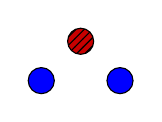
\begin{tikzpicture}
			\node[draw,fill=blue, circle] at (0,0) {};
			\node[draw,fill=blue, circle] at (1,0) {};
			\node[draw, circle, pattern=north east lines, pattern, preaction={fill=red}] at (0.5,0.5) {};
		\end{tikzpicture}
	\end{center}
	\newpage
	\begin{center}
		\begin{tikzpicture}[
				sibling distance=150pt,
				level distance=100pt,
				level 1/.style={sibling distance=6cm},
				level 2/.style={sibling distance=3cm},
				every node/.style = {
					shape=rectangle,
					rounded corners,
					draw,
					align=center,
				},
				every child/.style = {
					ultra thick
				}
			]
	\node {
		\begin{tikzpicture}
			\node[draw,fill=blue, circle] at (0,0) {};
			\node[draw,fill=blue, circle] at (1,0) {};
			\node[draw, circle, pattern=north east lines, pattern, preaction={fill=red}] at (0.5,0.5) {};
		\end{tikzpicture}
	}
		child [draw=blue] { node{
			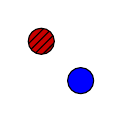
\begin{tikzpicture}
				\node[draw,fill=blue, circle] at (1,0) {};
				\node[draw, circle, pattern=north east lines, pattern, preaction={fill=red}] at (0.5,0.5) {};
			\end{tikzpicture}
		}}
		child [draw=red, densely dashed] { node{
			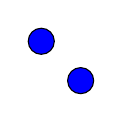
\begin{tikzpicture}
				\node[draw,fill=blue, circle, solid] at (1,0) {};
				\node[draw,fill=blue, circle, solid] at (0.5,0.5) {};
			\end{tikzpicture}
		}
	};
		\end{tikzpicture}
	\end{center}
	
	\newpage
	\begin{center}
		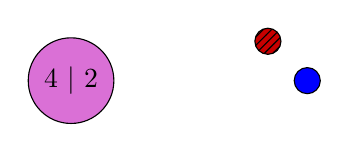
\begin{tikzpicture}
			\begin{scope} [every node/.style={style=circle, draw, fill=purple2}]
				\node at (-2,0) {4 $|$ 2};
				\node[draw,fill=blue, circle] at (1,0) {};
				\node[draw, circle, pattern=north east lines, pattern, preaction={fill=red}] at (0.5,0.5) {};
			\end{scope}
		\end{tikzpicture}
	\end{center}
	
		\newpage
	\begin{center}
		\begin{tikzpicture}[
			sibling distance=150pt,
			level distance=100pt,
			level 1/.style={sibling distance=6cm},
			level 2/.style={sibling distance=3cm},
			every node/.style = {
				shape=rectangle,
				rounded corners,
				draw,
				align=center,
			},
			every child/.style = {
				ultra thick
			}
			]
			\node {
				\begin{tikzpicture}
					\begin{scope} [every node/.style={style=circle, draw, fill=purple2}]
						\node at (-2,0) {4 $|$ 2};
						\node[draw,fill=blue, circle] at (1,0) {};
						\node[draw, circle, pattern=north east lines, pattern, preaction={fill=red}] at (0.5,0.5) {};
					\end{scope}
				\end{tikzpicture}
			}
			child [draw=blue] { node{
					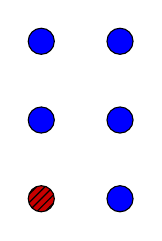
\begin{tikzpicture}
						\begin{scope} [every node/.style={style=circle, draw, fill=purple2}]
							\node[draw,fill=blue, circle] at (0,1) {};
							\node[draw,fill=blue, circle] at (0,2) {};
							\node[draw,fill=blue, circle] at (1,2) {};
							\node[draw,fill=blue, circle] at (1,1) {};
							\node[draw,fill=blue, circle] at (1,0) {};
							\node[draw, circle, pattern=north east lines, pattern, preaction={fill=red}] at (0,0) {};
						\end{scope}
					\end{tikzpicture}
			}}
			child [draw=red, densely dashed] { node{
					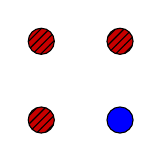
\begin{tikzpicture}
						\begin{scope} [every node/.style={style=circle, draw, fill=purple2, solid}]
							\node[draw, circle, pattern=north east lines, pattern, preaction={fill=red}] at (0,0) {};
							\node[draw, circle, pattern=north east lines, pattern, preaction={fill=red}] at (1,1) {};
							\node[draw,fill=blue, circle] at (1,0) {};
							\node[draw, circle, pattern=north east lines, pattern, preaction={fill=red}] at (0,1) {};
						\end{scope}
					\end{tikzpicture}
				}
			};
		\end{tikzpicture}
	\end{center}
	
	
	\newpage
	\begin{center}
		Qual o melhor lance para a esquerda?
		
		\vspace{1cm}
		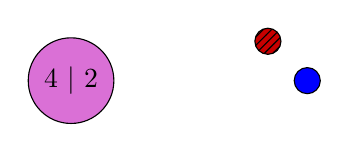
\begin{tikzpicture}
			\begin{scope} [every node/.style={style=circle, draw, fill=purple2}]
				\node at (-2,0) {4 $|$ 2};
				\node[draw,fill=blue, circle] at (1,0) {};
				\node[draw, circle, pattern=north east lines, pattern, preaction={fill=red}] at (0.5,0.5) {};
			\end{scope}
		\end{tikzpicture}
	\end{center}

	\newpage
	\begin{center}
		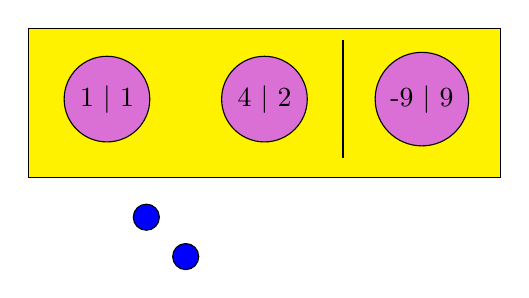
\begin{tikzpicture}
			\begin{scope} []
				\draw[fill=yellow] (-1,-1) rectangle ++(6,1.9);
				\node[circle, draw, fill=purple2] at (0,0) {1 $|$ 1};
				\node[circle, draw, fill=purple2] at (2,0) {4 $|$ 2};
				\draw[thick] (3,-0.75) -- (3,0.75);
				\node[circle, draw, fill=purple2] at (4,0) {{-}9 $|$ 9};
				\node[draw,fill=blue, circle] at (1,-2) {};
				\node[draw,fill=blue, circle] at (0.5,-1.5) {};
			\end{scope}
		\end{tikzpicture}
	\end{center}

	\newpage
	\begin{center}
		O melhor lance numa componente muda
		
		\vspace{1cm}
		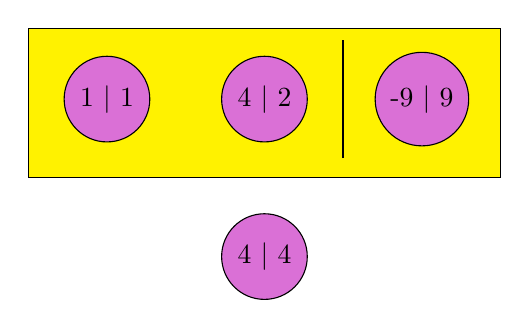
\begin{tikzpicture}
			\begin{scope} []
				\draw[fill=yellow] (-1,-1) rectangle ++(6,1.9);
				\node[circle, draw, fill=purple2] at (0,0) {1 $|$ 1};
				\node[circle, draw, fill=purple2] at (2,0) {4 $|$ 2};
				\draw[thick] (3,-0.75) -- (3,0.75);
				\node[circle, draw, fill=purple2] at (4,0) {{-}9 $|$ 9};
				\node[circle, draw, fill=purple2] at (2,-2) {4 $|$ 4};
			\end{scope}
		\end{tikzpicture}
	\end{center}

	\newpage
	\begin{center}
		Mas quais os parâmetros da mudança?
		
		\vspace{1cm}
		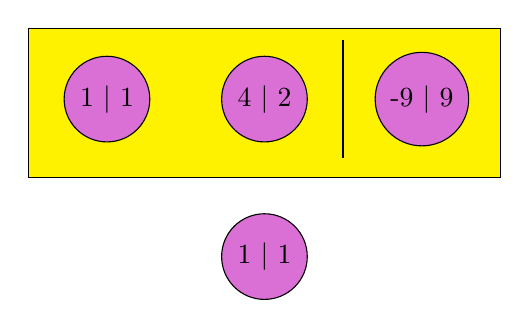
\begin{tikzpicture}
			\begin{scope} []
				\draw[fill=yellow] (-1,-1) rectangle ++(6,1.9);
				\node[circle, draw, fill=purple2] at (0,0) {1 $|$ 1};
				\node[circle, draw, fill=purple2] at (2,0) {4 $|$ 2};
				\draw[thick] (3,-0.75) -- (3,0.75);
				\node[circle, draw, fill=purple2] at (4,0) {{-}9 $|$ 9};
				\node[circle, draw, fill=purple2] at (2,-2) {1 $|$ 1};
			\end{scope}
		\end{tikzpicture}
	\end{center}

	\newgeometry{top=1cm}

	\newpage
	\begin{center}
		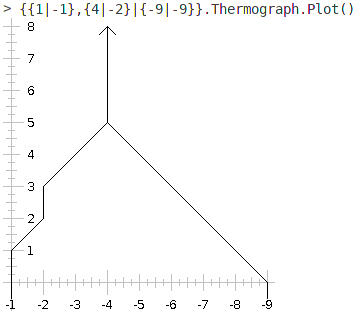
\includegraphics[scale=0.5]{g1Therm.png}
		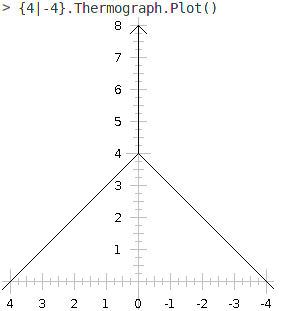
\includegraphics[scale=0.5]{g2Therm.png}
		
		\vspace{1cm}
		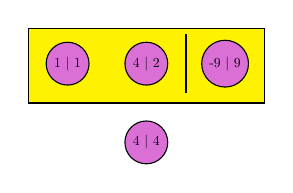
\begin{tikzpicture}[scale=0.5, every node/.style={scale=0.5}]
			\begin{scope} []
				\draw[fill=yellow] (-1,-1) rectangle ++(6,1.9);
				\node[circle, draw, fill=purple2] at (0,0) {1 $|$ 1};
				\node[circle, draw, fill=purple2] at (2,0) {4 $|$ 2};
				\draw[thick] (3,-0.75) -- (3,0.75);
				\node[circle, draw, fill=purple2] at (4,0) {{-}9 $|$ 9};
				\node[circle, draw, fill=purple2] at (2,-2) {4 $|$ 4};
			\end{scope}
		\end{tikzpicture}
	\end{center}
\end{document}
%----------------------------------------------------------------------------------------------------%
